\subsection{Korrespondenztabelle}
\thispagestyle{fancy}
Im täglichen Gebrauch wird die $\mu$SD-Karte mit allen Audiodateien einer Sprache beschrieben und muss somit an der Kasse nur noch mit einer Inventarliste der Audiodateien geladen werden.
In dieser Inventarliste wird vermerkt, welche Beacons zu welchen Audiodateien korrespondieren.
Befindet sich der Audioguide in einer Ausstellung, für die nicht bezahlt wurde, wird der Audioguide keine korrespondierende Audiodatei finden und signalisiert über die Lichtfugen, dass die Ausstellung zu verlassen ist.

Die Inventarliste wird an der Kasse über eine serielle Schnittstelle dem Mikrocontroller übergeben, der sie im EEPROM speichert.
Wird eine andere Sprache als die schon auf der microSD-Karte gespeicherte Sprache gefragt, kann die $\mu$SD-Karte mit einer anderen Sprache beschrieben werden, was jedoch circa eine Minute dauern kann.

Die Inventarliste wird von einer Textdatei erstellt, in der vermerkt wird, welcher Beacon zu welcher Ausstellung, Audiodatei und Textdatei gehört.
Diese Textdatei wird von der Software auf dem PC gelesen und über eine graphische Oberfläche kann das Kassenpersonal dem Audioguide die gewünschten Ausstellungen freischalten.

Am Ende des Besuchs werden die gelikeden Beacon-IDs wieder vom PC eingelesen und falls gewünscht kann ein persönliches Dokument mit den gelikeden Ausstellungsobjekten zusammengestellt werden.

\begin{figure}[H]
	\centering
	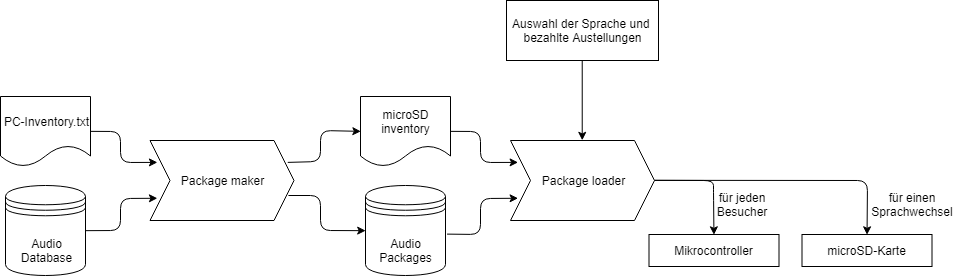
\includegraphics[width=\textwidth]{Bilder/data_flow.png}
	\caption{Data-Flow}
	\label{fig:data-flow}
\end{figure}

Auf dem PC werden die Audiodateien mit für den Nutzer sinnvollen Namen gepeichert, wobei eine Textdatei angibt, welche Audiodateien zu welchen Beacons und Ausstellungen gehören.
Diese Textdatei wird vom Nutzer erstellt und kann erweitert werden, sollte sich etwas an den Ausstellungen ändern.

Der Package-maker verwendet die Inventardatei um aus den Audiodateien sprachspezifische Pakete zusammenzustellen, jede mit einer sprachspezifischen Inventarsdatei.
Die Audiodateien in den Paketen sind nun umbenannt, damit sie in der richtigen Reihenfolge auf den Audioguide geladen werden können.
Die Inventarsdatei hat in derselben Reihenfolge eine Liste der Beacons, wobei jeder Beacon noch ein Datenfeld hat, das angibt, ob der Nutzer Zugriff auf das Ausstellungsobjekt hat und ob das Ausstellungsobjekt geliked wurde.
\newpage
